\section{Experimento 1: Red de Starbucks}

\subsection{Descripción del contexto}

El primer experimento fue realizado en una red inalambrica abierta de FibertelZone, por medio de una conexión Wi-Fi en una sucursal de la cadena Starbucks (ubicada en Avenida Corrientes esquina Malabia, en la ciudad autonoma de Buenos Aires, Republica Argentina) el dia Lunes 9 de Octubre de 2017. 
Al momento de comenzar las mediciones, se observo que dentro de la red se encontraban conectadas 10 notebooks y varios dispositivos mobiles (se estima uno por persona) , además del router propio del local. Considerando aproximadadmente 30 personas en el lugar contamos con 41 dispositivos conectados. 

\subsection{Descripción de la captura}

La captura resulto en un total de 12000 paquetes. La figura~\ref{protocolos1} muestar la distribucion de los protocolos de los paquetes capturados. Se puede ver claramente que la mayoria de los paquetes son de tipo Ipv4, mientras que en menor medida encontramos paquetes de tipo Ipv6 (0x86dd) y un menor porcentaje de paquetes ARP. 
Los dos primeros son distintas versiones del protocolo Ip (nivel de redes dentro del modelo OSI), mientras que el ultimo es un protocolo utilizado por los dispositivos para llenar su tabla de drecciones MAC, ya que cada dispositivo necesita para mandar correctamente un paquete cual es la direccion local (MAC) correspondiente a una direccion Ip. 
Resulta esperable que la mayoria de los paquetes sean del protocolo Ip, ya que es el utilizado para el intercambio de datos. Sin embargo, consideramos tambien (comparativamente) relevante la cantidad de paquetes ARP, lo cual atribuimos a la gran cantidad de dispositivos conectados en la red analizada.

\begin{figure}[H]
\centering
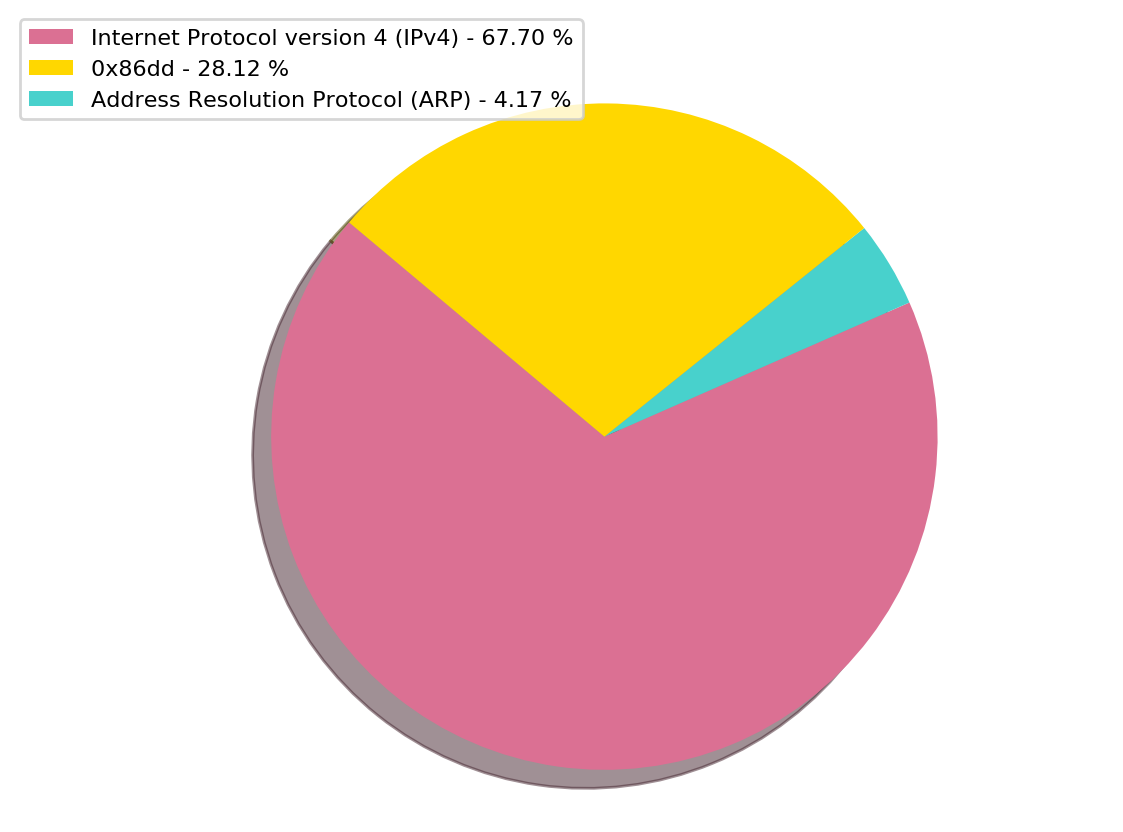
\includegraphics[width=0.7\textwidth]{protocolosRed1.png}
\caption{Gráfico que muestra la distribución de protocolos en la red.}
\label{protocolos1}
\end{figure}

En la figura~\ref{broadcast1} comparamos el porcentaje de paquetes broadcast contra el porcentaje de paquetes unicast. Un paquete bradcast es aquel cuya direccion destino tiene un valor especial, el cual al ser recibido siempre se considera correspondiente ( a diferencia de un paquete unicast donde sera considerado correspondiente cuando la direccion destino coincida con la propia). En este caso observamos que los paquetes broadcast representan el 16% del total.
Como muestra la figura~\ref{entropias1_1}, los protocolos con mensajes broadcast son Ipv4 y ARP, siendo estos ultimos del tipo who-has. Este tipo de mensaje corresponde a un pedido dirigido a todos en la red solicitando la direccion MAC de una Ip determinada.

\begin{figure}[H]
\centering
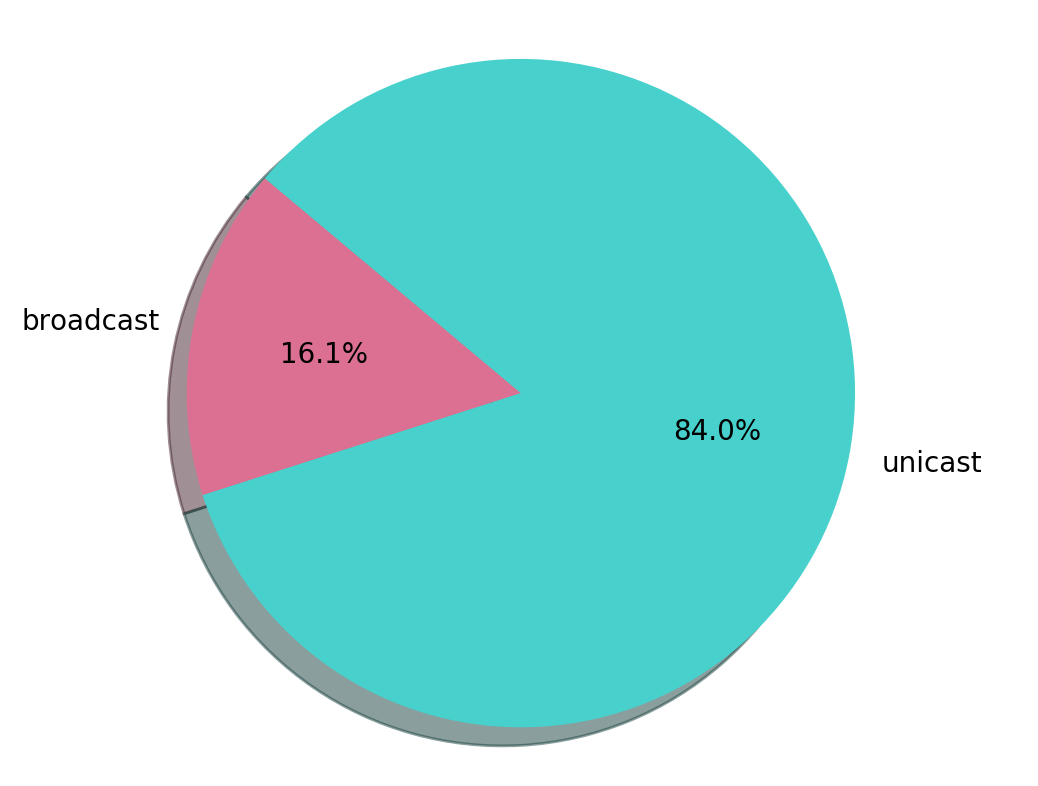
\includegraphics[width=0.7\textwidth]{broadcastRed1.png}
\caption{Gráfico que muestra los porcentajes de tráfico broadcast y unicast.}
\label{broadcast1}
\end{figure}

\subsection{Análisis de la captura}

El modelado de la fuente S1 fue realizado siguiendo las especificaciones de la consigna.
En la figura 3 se puede observar que separamos a los paquetes por su protocolo y por si son broadcast o unicast y calculamos su informacion. Incluimos tambien la entropia maxima y la entropia muestral.
La probabilidad de aparicion de un simbolo es inversamente proporcional a su informacion.
Para esta captura particular el símbolo con más información es representado por los paquetes unicast de tipo ARP. Estos paquetes son los is-at ( las respuestas a los who-has). 

El símbolo con más información (ARP unicast) tiene aproximadamente 10
veces la información del menor (IPv4 unicast). Notese que  segun la teoria de la informacion, la entropía máxima se alcanza cuando la información de todos los símbolos es la misma.

\begin{figure}[H]
\centering
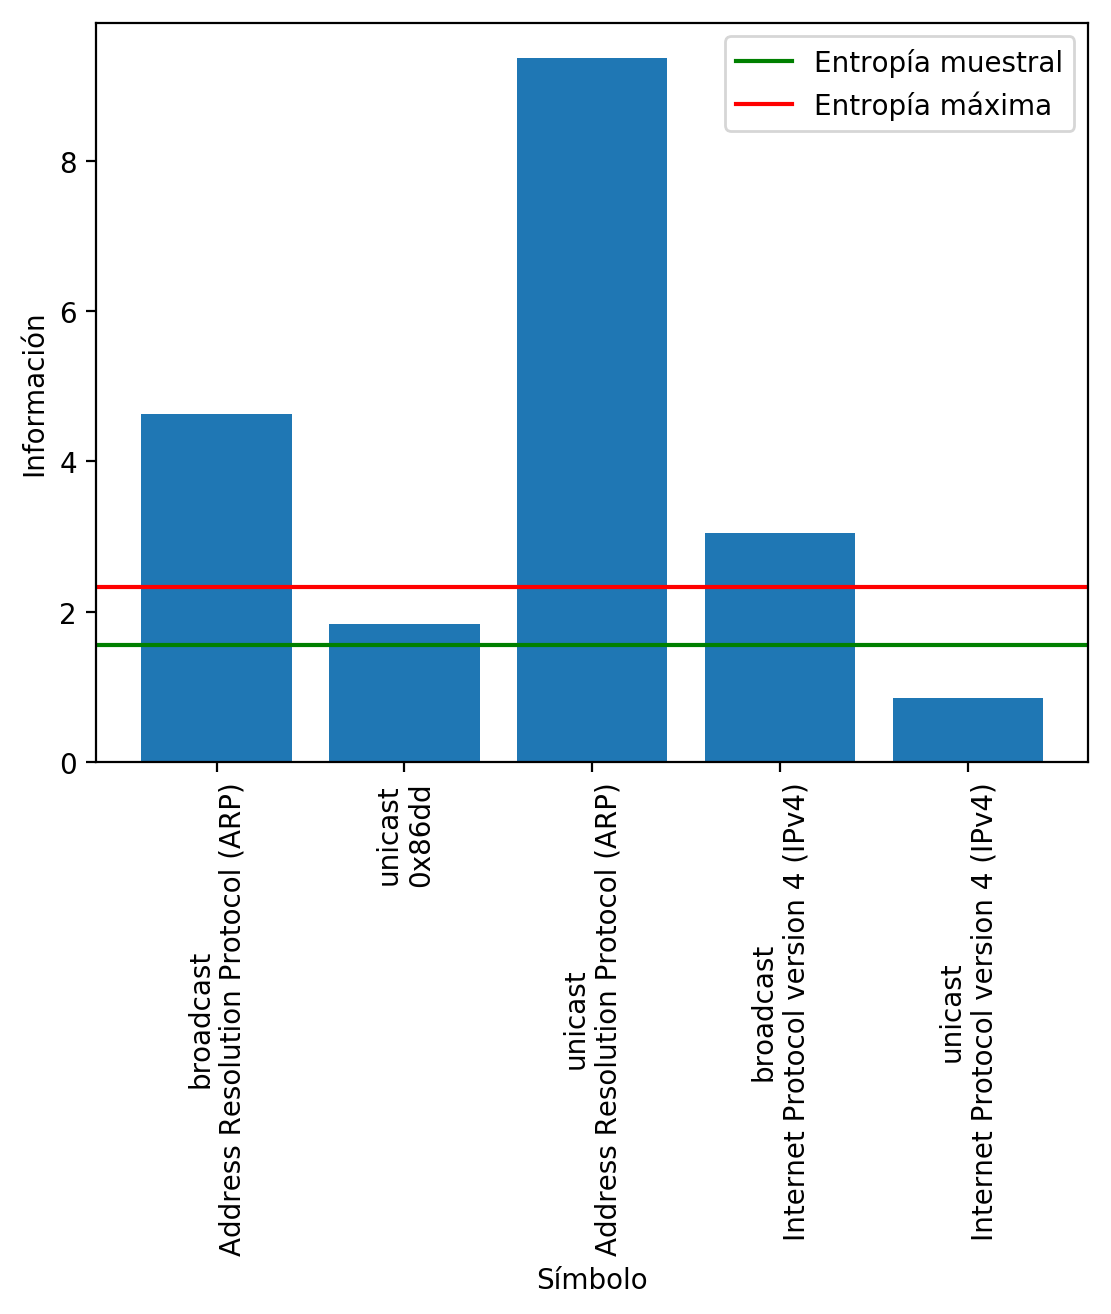
\includegraphics[width=0.7\textwidth]{entropiaS1Red1.png}
\caption{Gráfico de la información de los símbolos de la fuente $S_1$ observados en esta red. Se muestra la entropía muestral de $S_1$ y su entropía máxima.}
\label{entropias1_1}
\end{figure}

El análisis usando el modelado de la fuente S2 (explicado anteriormente) se puede ver en la figura 4. En este caso notamos que los símbolos de la fuente podrían dividirse en 2 o 3 grupos de acuerdo a su información. 
Se observan algunos puntos distinguidos, en particular las 8 IPs con información menor a la entropía de S2. Estas son las IPs que más requests ARP hicieron. 

La entropía muestral es aproximadamente 4/5 de la máxima. Encontramos que este nivel se debe a la presencia de varios símbolos con valores de información similares (nuevamente, la máxima entropia se alcanza con equiprobabilidad).

\begin{figure}[H]
\centering
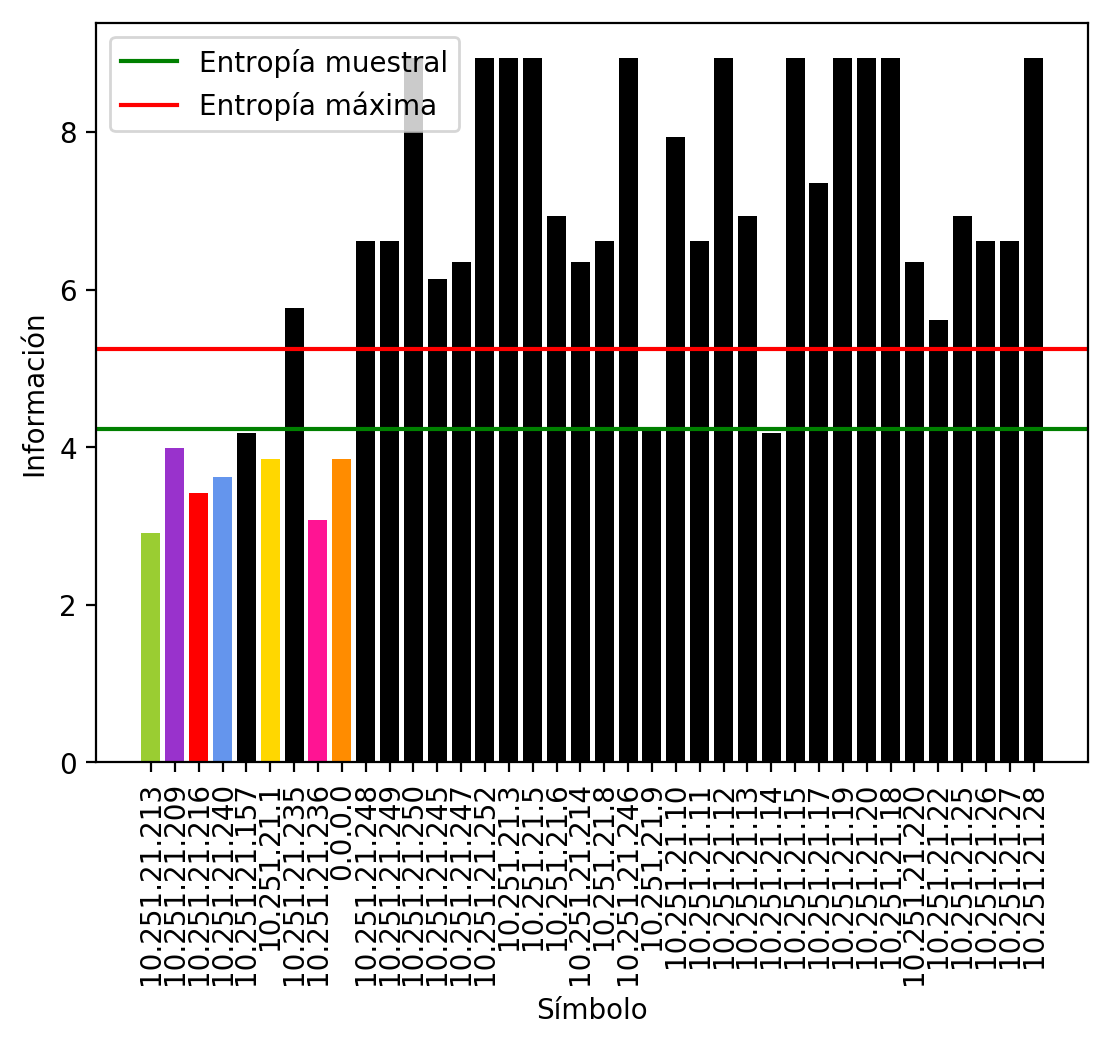
\includegraphics[width=0.7\textwidth]{entropiaS2Red1.png}
\caption{Gráfico de la información de los símbolos de la fuente $S_2$ observados en esta red. Se muestra la entropía muestral de $S_2$ y su entropía máxima.}
\label{entropias2_1}
\end{figure}

Por último graficamos la red subyacente de mensajes ARP representandola en la figura 5. 
Cada nodo del grafo representa una IP interviniente en al menos un mensaje ARP de la red, y cada eje orientado representa que un nodo (con su correspondiente Ip) envió al menos un mensaje con Ip destino correspondiente al nodo apuntado, sin distinguir entre paquetes de tipo who-has o is-at.

Dada esta representacion, es importante leer correctamente el grafico, ya que los nodos con mayor grado no son necesariamente los de mayor probabilidad. 
Dada una Ip origen, puede haber un caso en que mande una gran cantidad de mensajes a unas pocas direcciones destino (recordar que en esta fuente se cuentan la cantidad de mensajes enviados osea las aristas que salen de cada nodo). 
Como este grafo no posee peso en las aristas, estos intercambios resultarian en un nodo con pocas aristas, mientras que otro intercambio de mensajes donde una ip destino manda comparativamente menos paquetes pero a una mayor cantidad de IPs distintas, resultara en un nodo con muchas mas aristas.
Teniendo en cuenta esto podemos notar que igualmente las direcciones con menor informacion (osea mayor probabilidad ) resultan las de mayor grado en el grafo.

\begin{figure}[H]
\centering
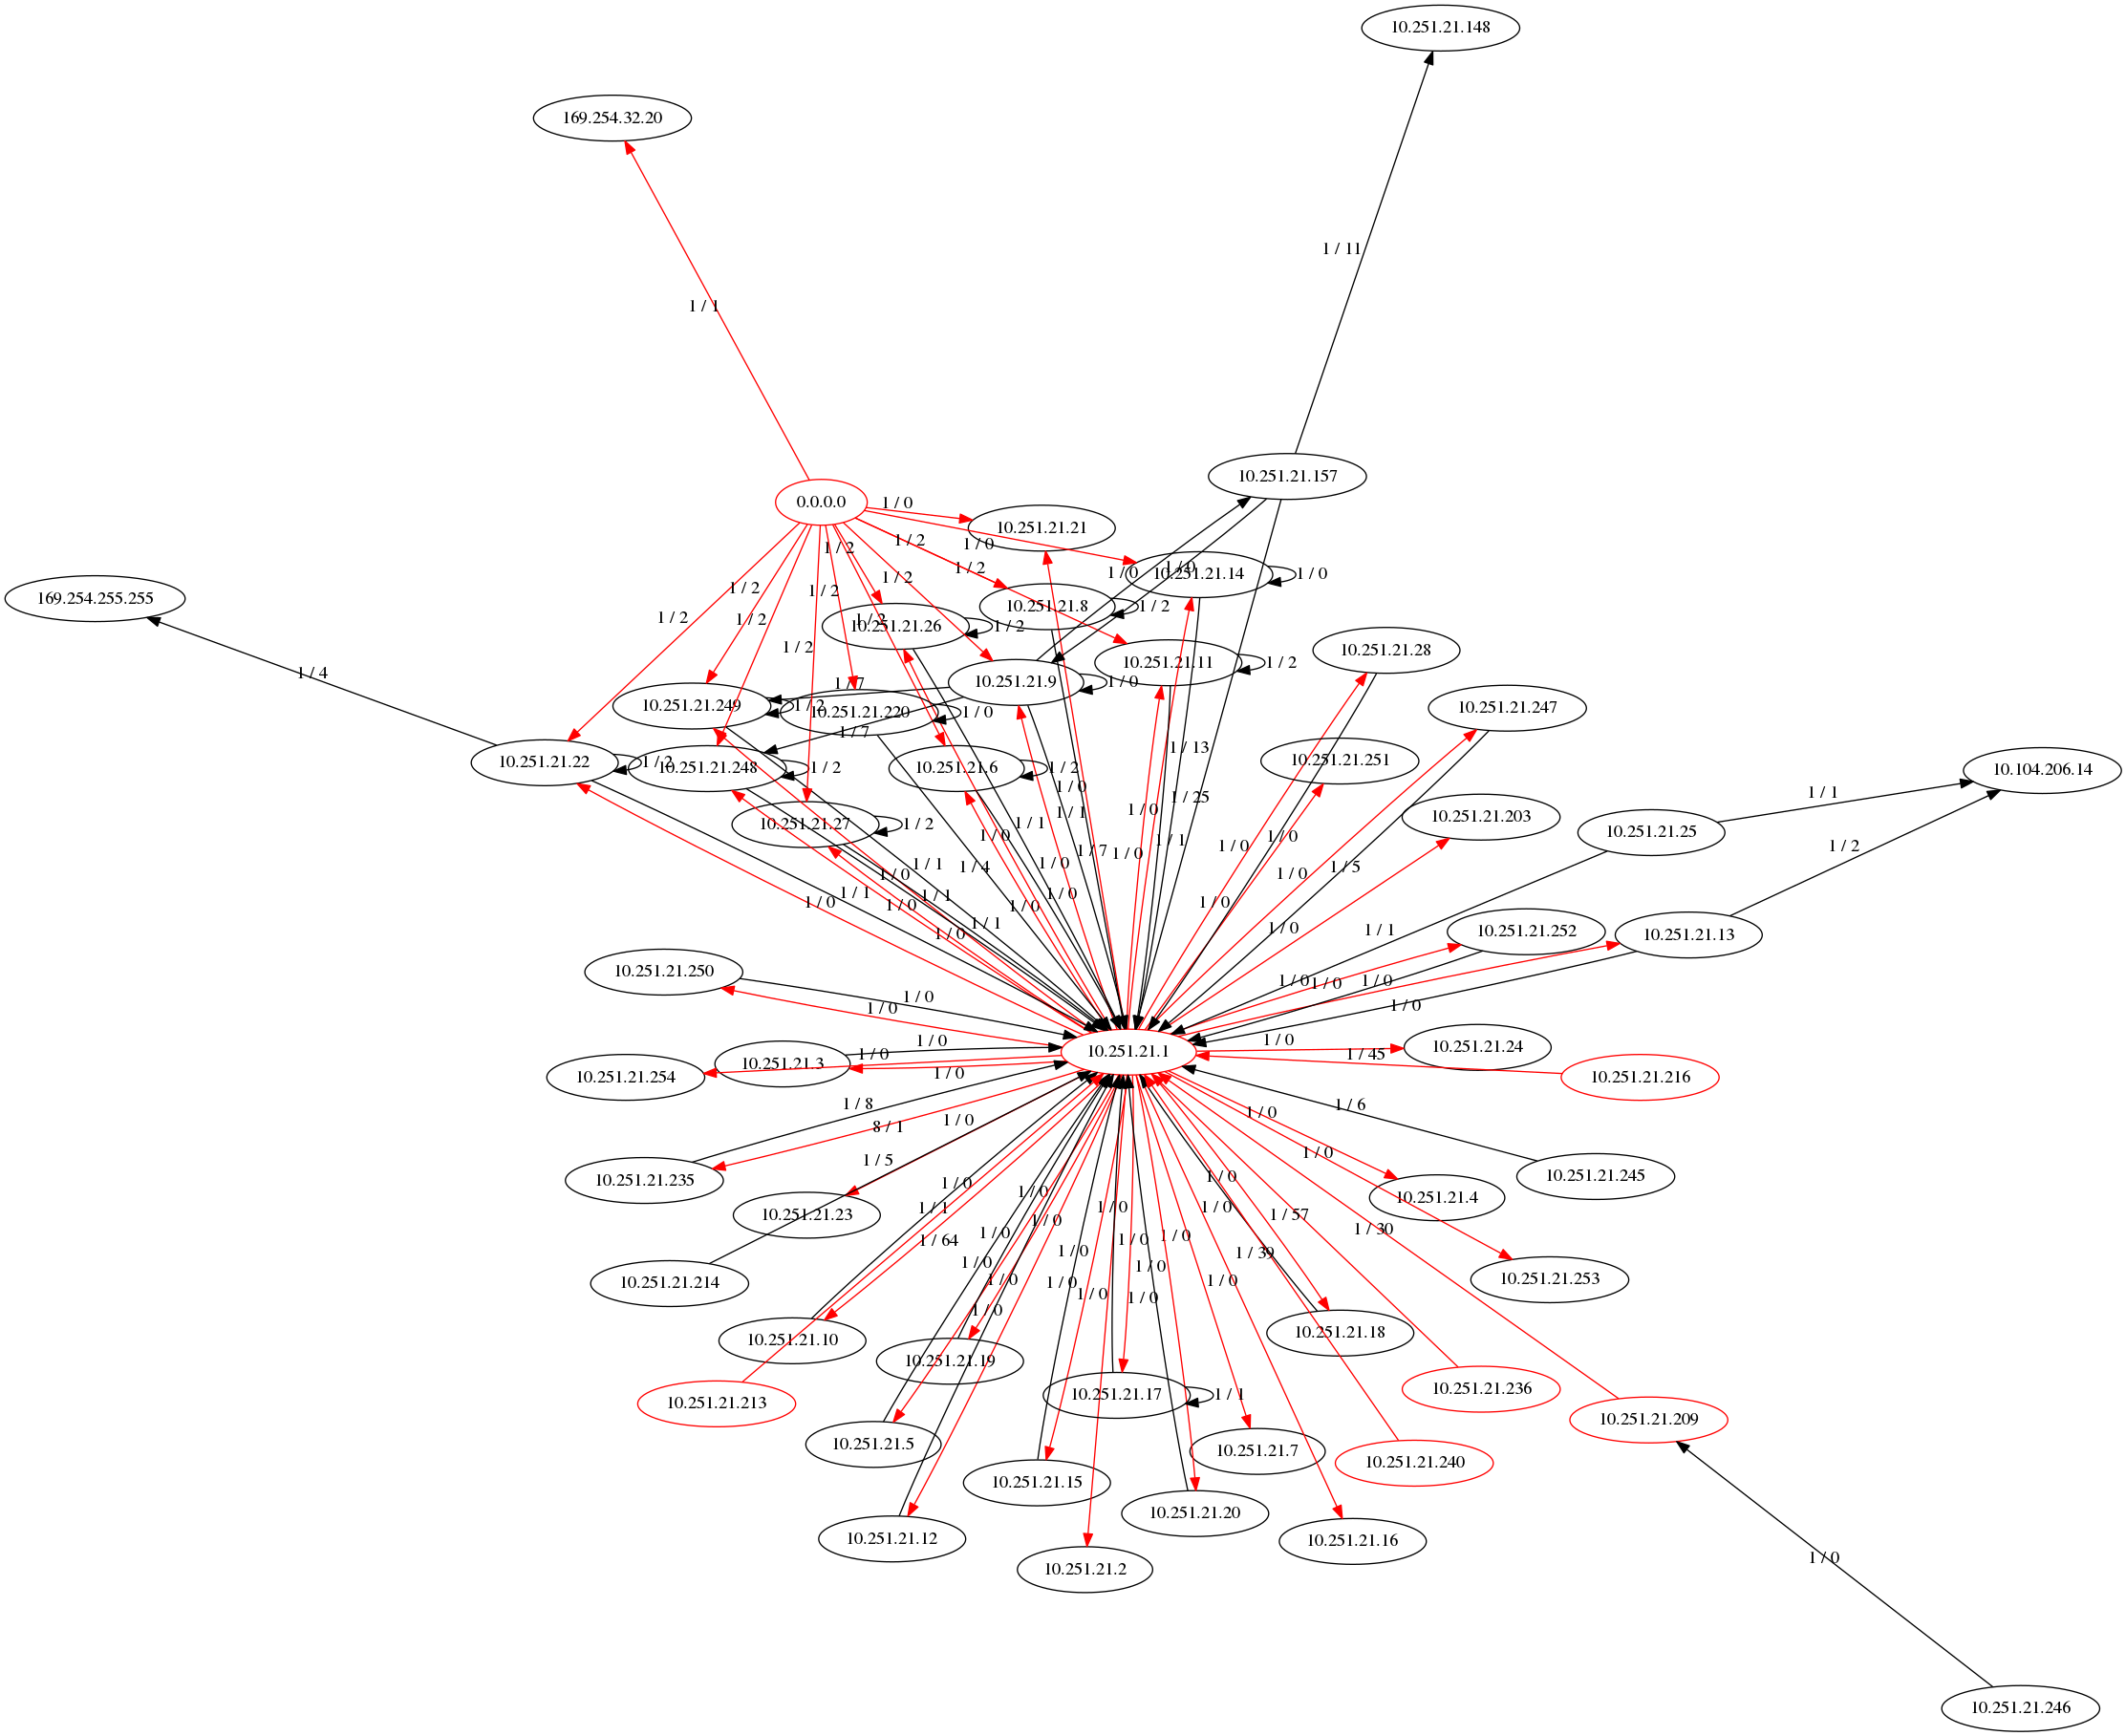
\includegraphics[width=\textwidth]{grafoRed1.png}
\caption{Grafo de la red de mensajes ARP subyacente. Los nodos son las IPs observadas y los ejes son los mensajes ARP. En colores se marcan los nodos distinguidos (información por debajo de la entropía) y sus mensajes salientes. Cada arista tiene anotada la cantidad de requests/replies ARP.}
\label{grafo1}
\end{figure}